\documentclass[11pt]{article}

\usepackage[margin=1in]{geometry}
\usepackage{amsmath}
\usepackage{graphicx}
\usepackage{booktabs}
\usepackage{float}
\usepackage{times}

\title{Finding Change Points by Optimization\\
\large Replacing the heuristic cascade with a single objective}
\author{Yuli Tshuva}
\date{September 2026}

\begin{document}
\maketitle

\section{The problem}

The old change point detector was a chain of local decisions. It looked at the
sign of the derivative, then filtered by prominence, then merged points that were
close together, then dropped points that had the same direction on both sides.
Each step had its own threshold: \texttt{SEGMENT\_PERCENTAGE},
\texttt{CHANGE\_THRESHOLD}, \texttt{MIN\_DISTANCE\_BETWEEN\_FEATURE\_POINTS},
a prominence of 5\% of the amplitude, a merge rule at 1\% of the amplitude, a
smoothing window.

Two things are wrong with this. First, there are six knobs and no principled way
to set any of them. Second, and worse, the steps run in order, so the result
depends on that order. A point dropped early can never come back. There is no
sense in which the answer is the best answer --- it is just the answer that
falls out of this particular pipeline.

\section{The idea}

Say instead what a \emph{good} segmentation is, and then find the best one.

Let the sequence have $n$ points. A segmentation is a set of cut positions
$0 = t_0 < t_1 < \dots < t_K = n$. Give every segment a cost $c(a,b)$, meaning
``how badly does a simple model explain the piece $y_{a:b}$''. Then solve

\begin{equation}
\min_{K,\; t_1 < \dots < t_{K-1}} \quad
\sum_{k=0}^{K-1} c(t_k,\, t_{k+1}) \;+\; \beta K .
\label{eq:main}
\end{equation}

The first term wants many short segments, because short pieces are easy to
explain. The term $\beta K$ pushes back: every extra cut costs $\beta$. The
balance between them decides how many change points there are.

This is solved \emph{exactly}, not approximately, by dynamic programming. Let
$F(t)$ be the best cost for the first $t$ points. Then

\begin{equation}
F(t) \;=\; \min_{s < t} \; \Big[ F(s) + c(s,t) + \beta \Big],
\qquad F(0) = 0,
\label{eq:dp}
\end{equation}

and the cuts are read back by following which $s$ won at each $t$. This is
$O(n^2)$, and it runs in about $0.1$ seconds for $n = 1000$.

Everything the old code did in a cleanup pass now lives inside
Equation~\eqref{eq:dp} as a constraint. A minimum segment length becomes
$s \le t - m$ in the search. A fixed number of change points becomes a second
table $C(k,t)$ instead of a penalty. A rule like ``no two neighbouring segments
may go the same way'' becomes an extra state. In every case the constraint is
respected \emph{and} the answer is still globally optimal --- which the
order-dependent merging passes could never promise.

\section{What is a segment cost?}

Two choices are implemented.

\paragraph{Straight-line cost.} Fit a least-squares line to the piece and take
the leftover error:
\begin{equation}
c(a,b) \;=\; \min_{\alpha,\gamma} \sum_{t=a}^{b-1} \big( y_t - \alpha - \gamma t \big)^2 .
\end{equation}
This says ``a segment is a trend'', which is exactly what a node in the graph is
meant to be.

\paragraph{Feature cost.} The distance function compares segments through a
feature vector $\phi$, using weights $w$ that were already tuned. Four of those
features --- mean value, mean slope, mean absolute slope, mean curvature --- are
simply the averages of four pointwise signals. Write that pointwise vector as
$\psi(t)$ and ask each segment to be flat in \emph{that} space:
\begin{equation}
c(a,b) \;=\; \sum_{t=a}^{b-1} \big\lVert\, w \odot \big( \psi(t) - \bar{\psi}_{a:b} \big) \big\rVert^2 ,
\qquad
\bar{\psi}_{a:b} = \frac{1}{b-a}\sum_{t=a}^{b-1} \psi(t).
\end{equation}
Now the segmentation is chosen in the same space, with the same weights, that
the similarity metric later measures. That is the honest meaning of ``change
point detection driven by the metric''.

Both costs are sums of squares, so with prefix sums of $y$, $y^2$, $ty$, $t$,
$t^2$ (and of $\psi$, $\psi^2$) each $c(a,b)$ is computed in constant time. That
is why the whole thing is fast.

\section{The one remaining knob}

Only $\beta$ is left. The textbook choice is a BIC penalty,
$\beta = 2\hat{\sigma}^2 p \log n$. On this data it fails: the sequences are
smoothed with a window of $5$ and stretched to $1000$ points, so the estimated
noise $\hat\sigma^2$ is almost zero, $\beta$ is almost zero, and the method
returns sixty or more change points.

So $\beta$ is set relative to the sequence itself:
\begin{equation}
\beta \;=\; \beta_{\mathrm{rel}} \cdot c(0,n).
\end{equation}
In words: a new cut is worth making only if it removes at least
$\beta_{\mathrm{rel}}$ of the error you would have with no cuts at all. This is
a pure number, comparable across sequences, and it is the single quantity to
tune against what we actually care about --- agreement with human similarity
judgements.

Figure~\ref{fig:beta} shows what it does. The result is stable: $K=4$ holds over
the whole range $\beta_{\mathrm{rel}} \in [0.01, 0.05]$, so this is a broad
plateau and not a knife edge.

\begin{figure}[H]
\centering
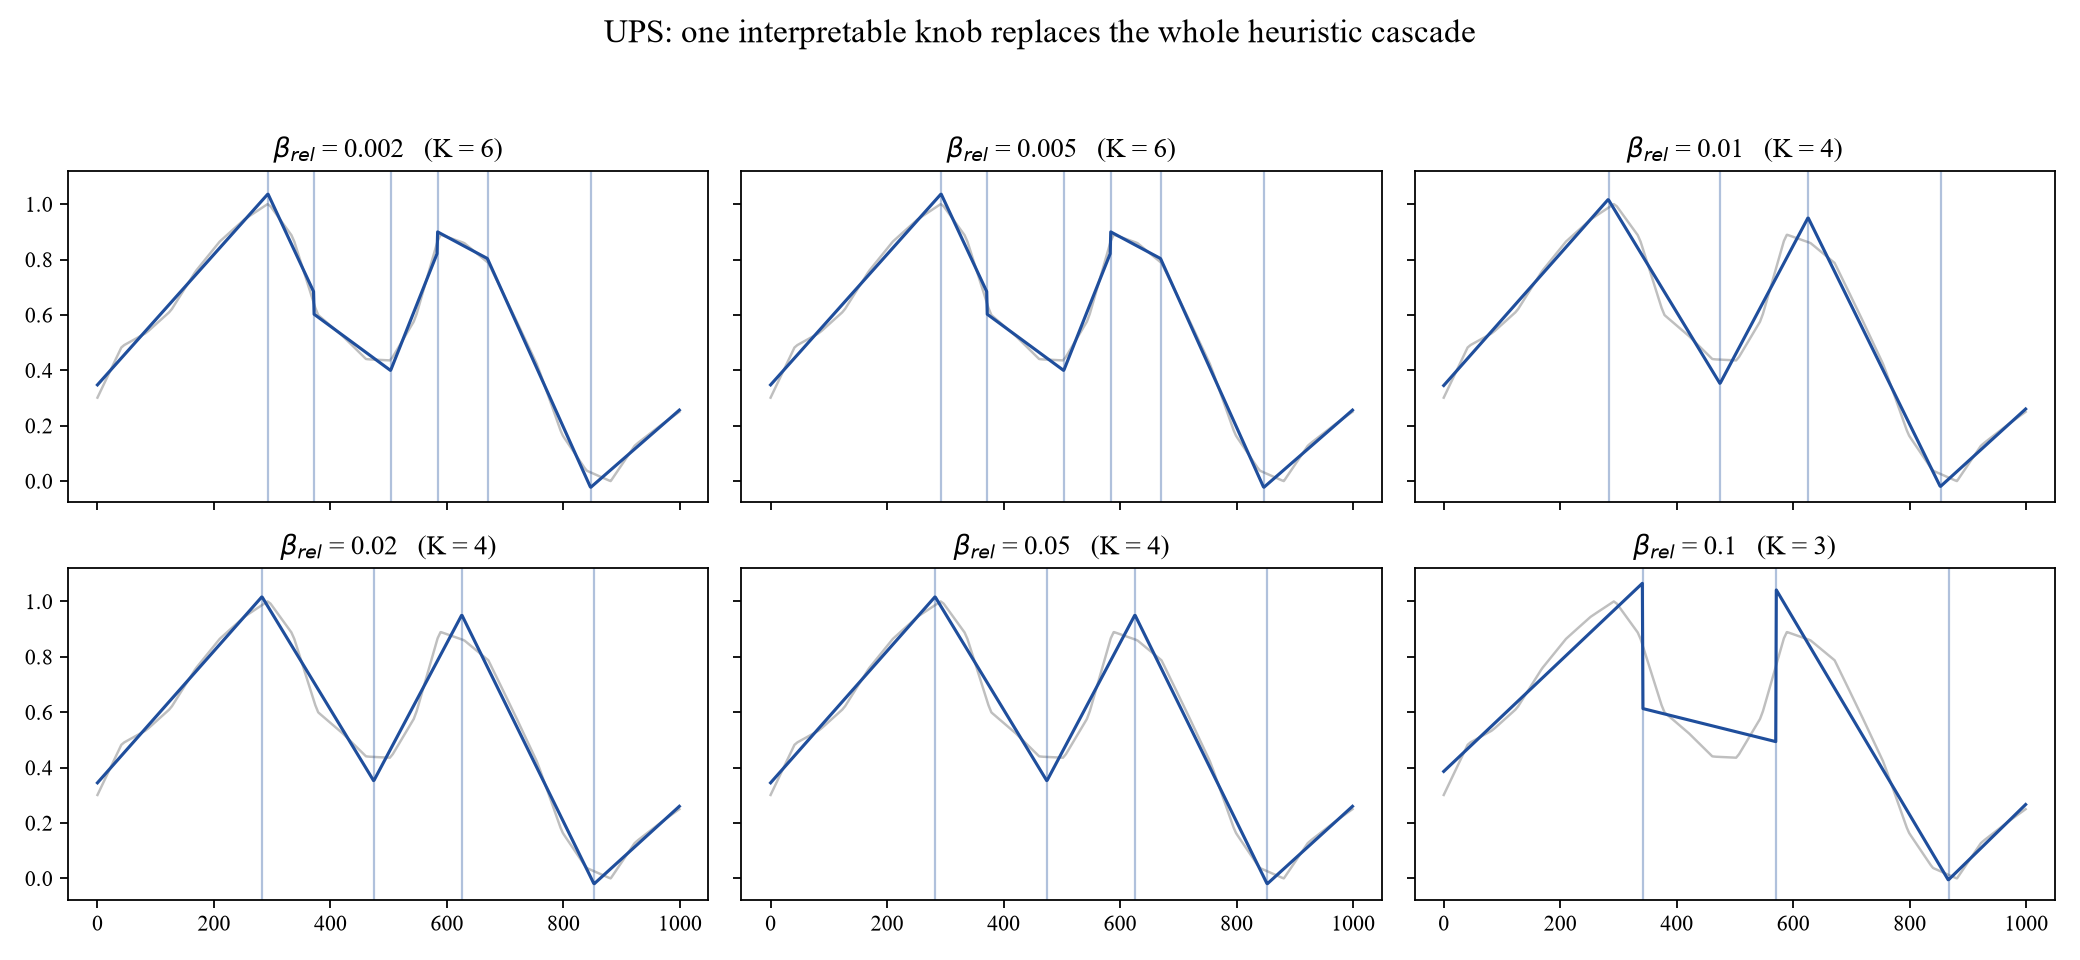
\includegraphics[width=\textwidth]{figs/cpd_opt_beta_sweep.png}
\caption{One interpretable knob replaces six thresholds. Small
$\beta_{\mathrm{rel}}$ buys more segments, large $\beta_{\mathrm{rel}}$ buys
fewer, and the middle range is flat.}
\label{fig:beta}
\end{figure}

\section{How it turns out}

Figure~\ref{fig:examples} shows what the method returns on six stocks: the
sequence, with the change points marked on it.

The cuts land where a reader would put them --- on the turns, at the tops and
bottoms, and where a steady climb changes its rate. Nothing is placed inside a
stretch that is already going one way, and no turn is left unmarked.

\begin{figure}[htbp]
\centering
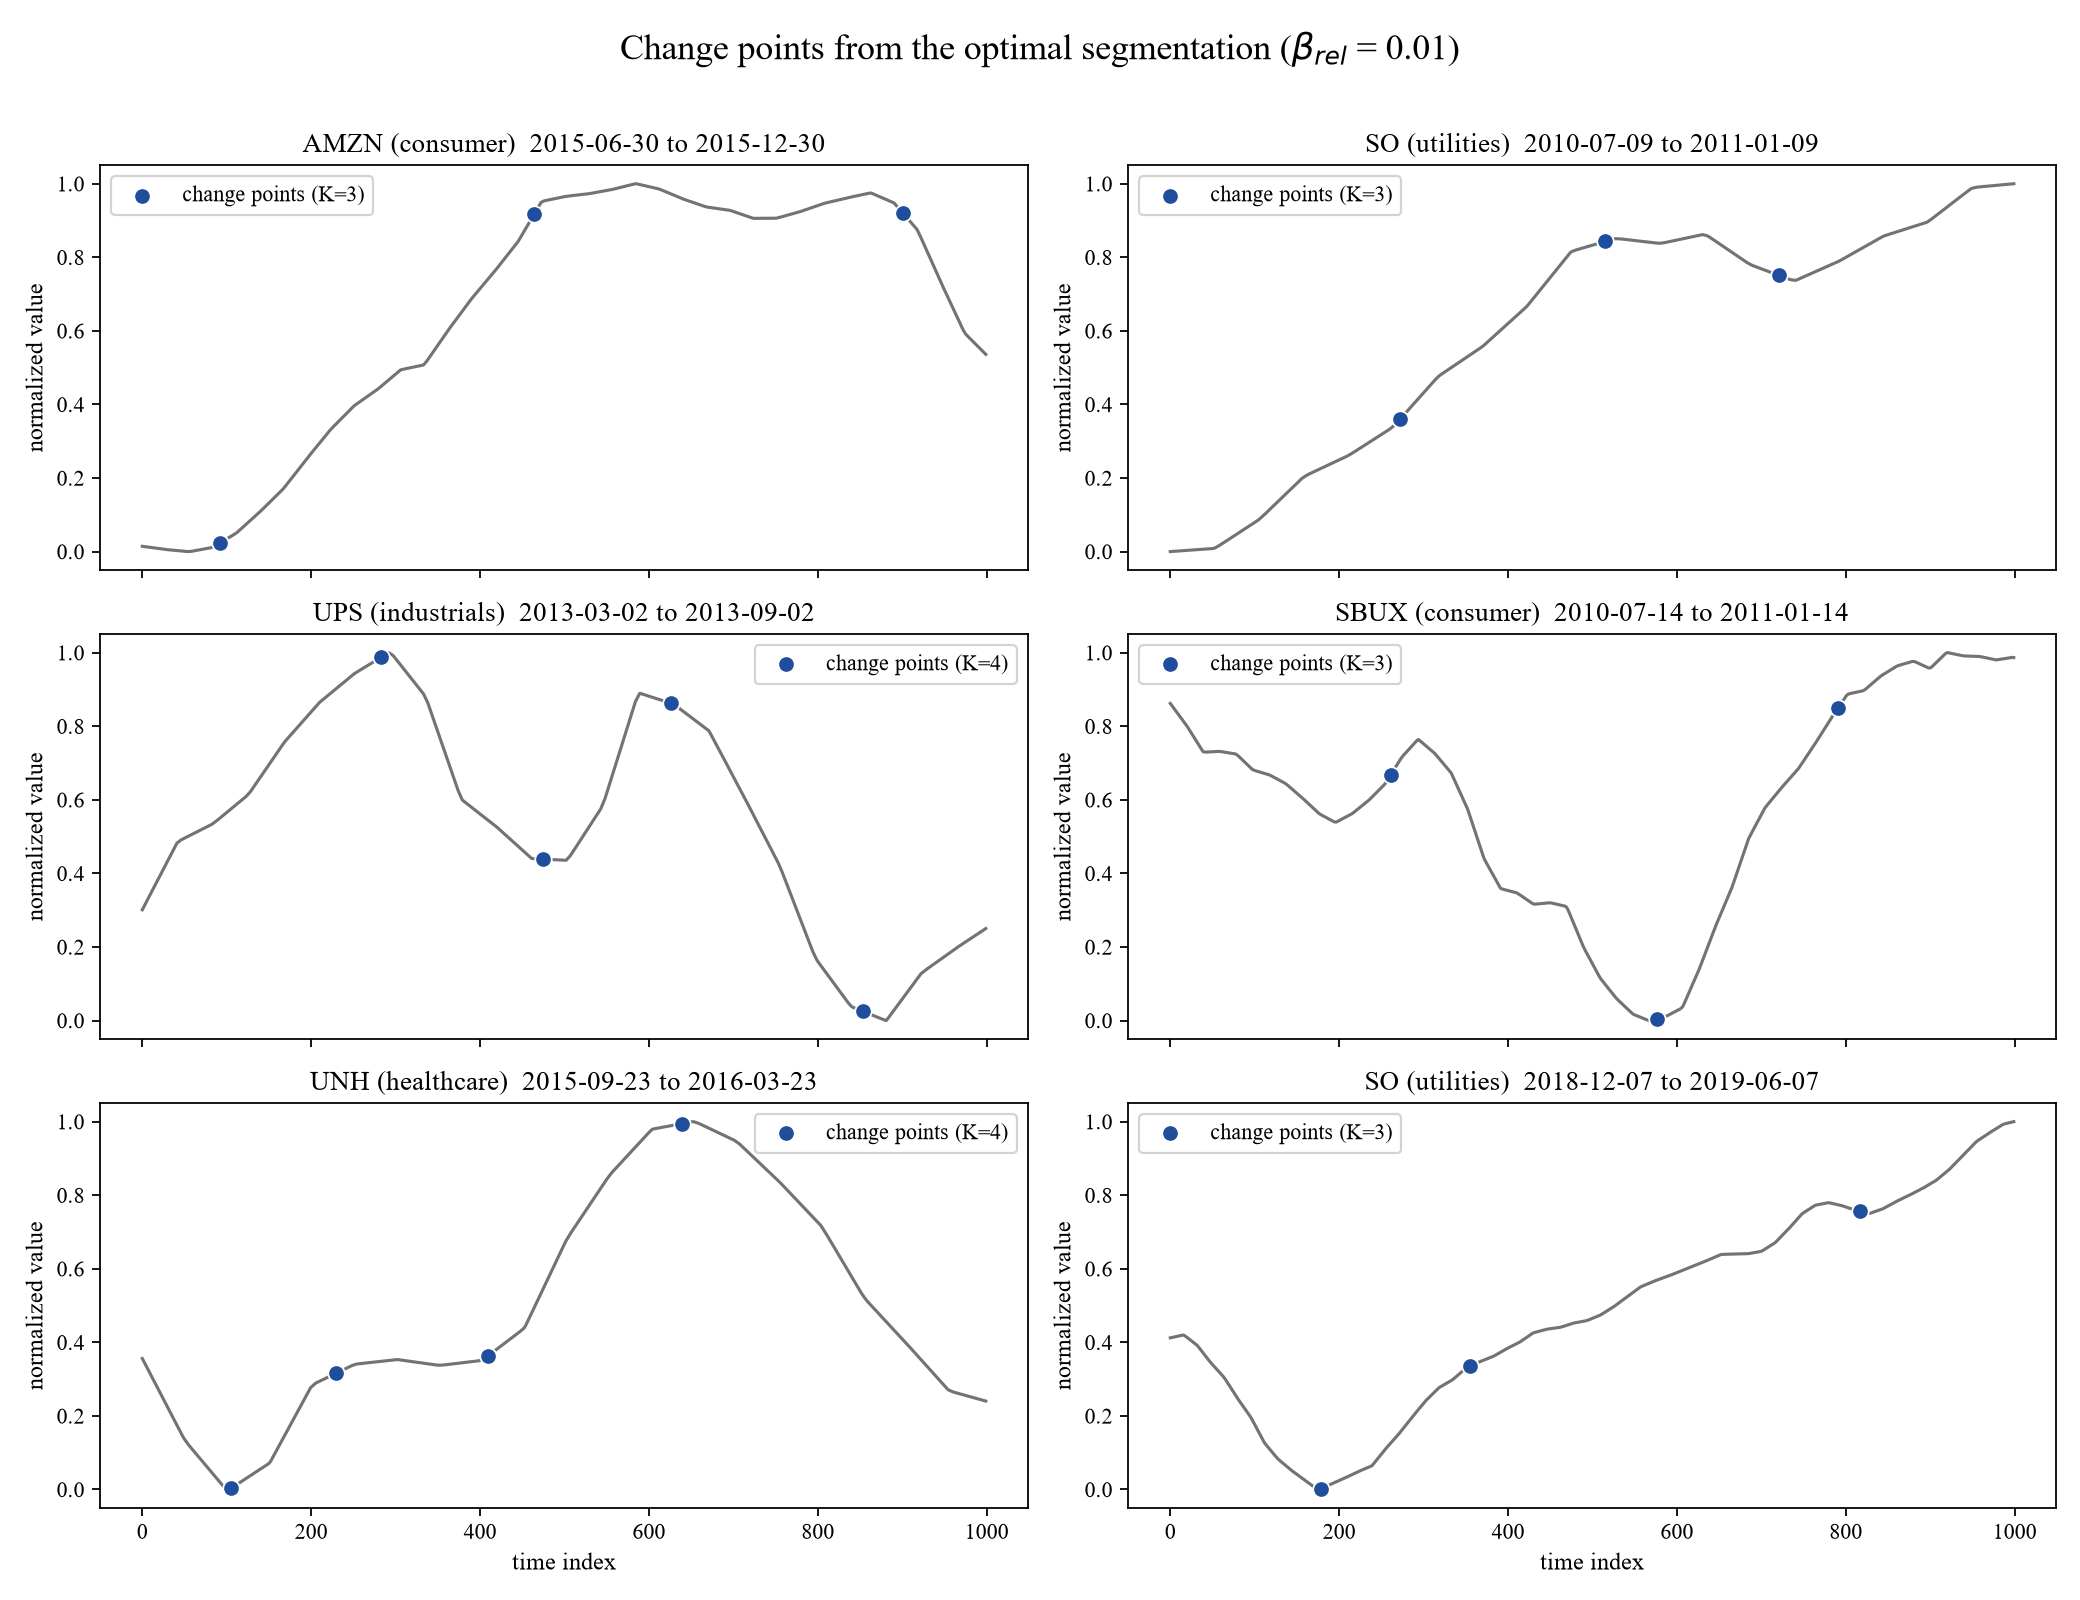
\includegraphics[width=\textwidth]{figs/cpd_opt_examples.png}
\caption{Six stocks with the change points found by the dynamic program at
$\beta_{\mathrm{rel}} = 0.01$.}
\label{fig:examples}
\end{figure}

Table~\ref{tab:sse} compares the two methods as a number. For each stock the
dynamic program was given the \emph{same} number of change points the heuristic
chose, so the comparison is fair. It removes between a third and four fifths of
the leftover error, on the same budget.

\begin{table}[H]
\centering
\caption{Reconstruction error at an equal number of change points.}
\label{tab:sse}
\begin{tabular}{lrrrr}
\toprule
Stock & $K$ & Heuristic & Optimal & Error removed \\
\midrule
AMZN & 4 & 0.761 & 0.288 & 62\% \\
SO   & 4 & 0.403 & 0.116 & 71\% \\
UPS  & 4 & 1.475 & 0.993 & 33\% \\
SBUX & 3 & 7.014 & 1.490 & 79\% \\
UNH  & 4 & 1.206 & 0.688 & 43\% \\
SO (2018) & 4 & 0.716 & 0.167 & 77\% \\
\bottomrule
\end{tabular}
\end{table}

Figure~\ref{fig:costk} is the same statement without picking a $K$. The blue
curve is the lowest error reachable with $K$ cuts --- by construction nothing
can go below it. The heuristic sits well above it.

\begin{figure}[htbp]
\centering
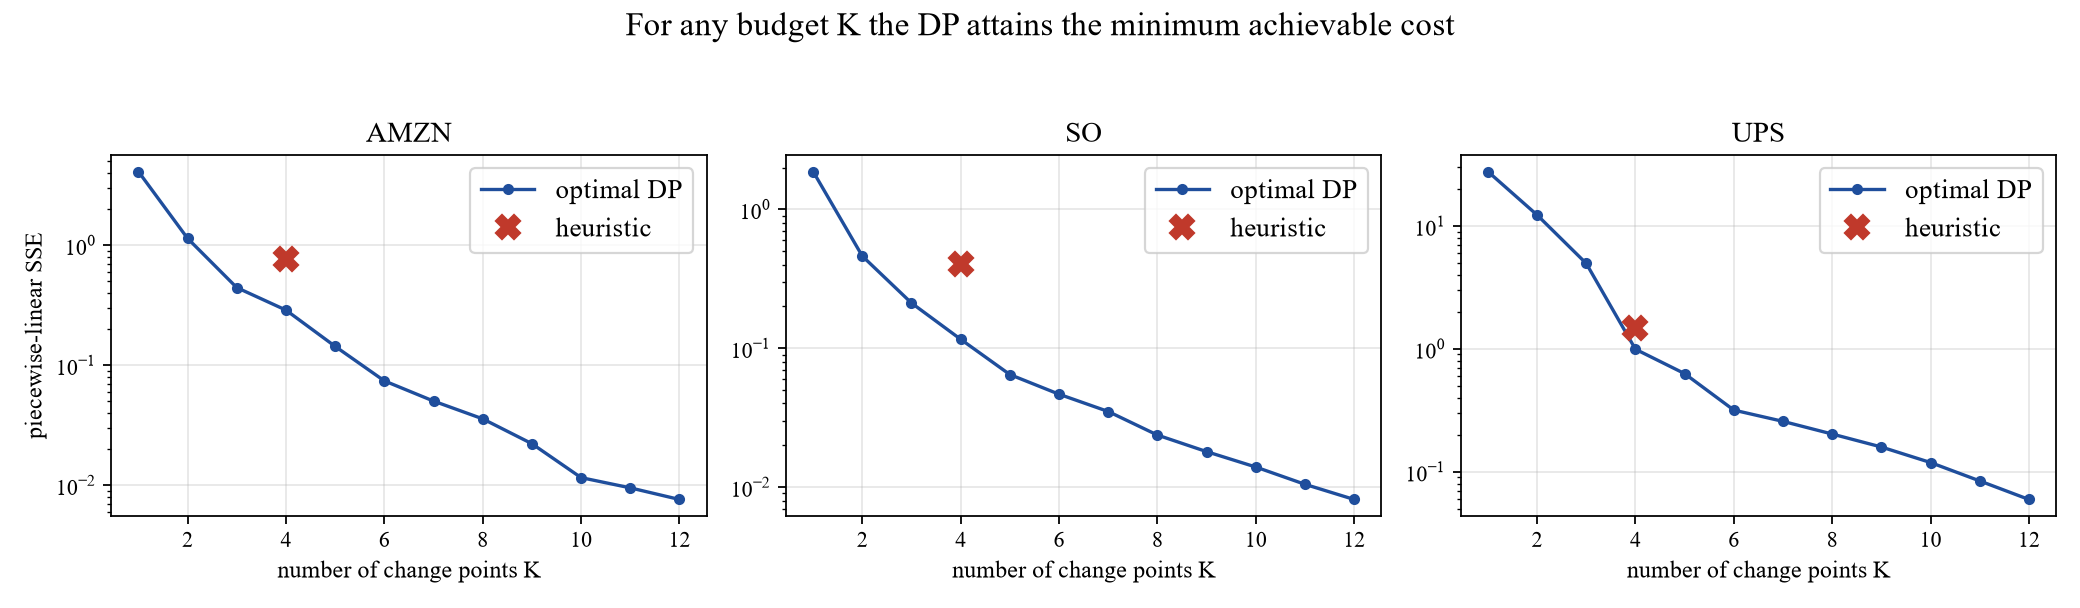
\includegraphics[width=\textwidth]{figs/cpd_opt_cost_vs_k.png}
\caption{Best achievable error against the number of change points. The
heuristic (red cross) is above the optimal curve at its own budget.}
\label{fig:costk}
\end{figure}

\section{What this does not yet show}

Low reconstruction error is the dynamic program's own objective, so it wins that
by definition. It is \emph{not} evidence that the similarity metric got better.
That claim needs the triplet data from the human study: sweep
$\beta_{\mathrm{rel}}$, measure agreement with human judgements, and compare
against the heuristic. That is the next step, and it is the point at which the
segmentation really becomes ``optimized for the metric''.

\section{Where the code is}

\sloppy
\begin{itemize}
\itemsep2pt
\item \texttt{cpd\_opt.py} --- the two costs, the penalized dynamic program, and
the fixed-$K$ version. The entry point
\texttt{optimal\_change\_points()} returns boundaries in the same format as the
old \texttt{change\_points\_detection()}, so it is a drop-in replacement.
\item \texttt{demo\_cpd\_opt.py} --- produces the three figures above and the table.
\end{itemize}

\end{document}
